\everymath{\displaystyle}
\documentclass{beamer}
% \documentclass[handout]{beamer}

%\usepackage[pdftex]{color,graphicx}
\usepackage{amsmath,amssymb,amsfonts}

\mode<presentation>
{
  % \usetheme{Darmstadt}
  % \usetheme[hideothersubsections]{Hannover}
  % \usetheme[hideothersubsections]{Goettingen}
  \usetheme[hideothersubsections, right]{Berkeley}

  \usecolortheme{seahorse}
  % \usecolortheme{dolphin}
  \usecolortheme{rose}
  % \usecolortheme{orchid}

  \useinnertheme[shadow]{rounded}

  \setbeamercovered{transparent}
  % or whatever (possibly just delete it)
}

\mode<handout>{
  \setbeamercolor{background canvas}{bg=black!5}
  \usepackage{pgfpages}
  \pgfpagesuselayout{4 on 1}[a4paper,border shrink=5mm, landscape]
}

\usepackage[brazilian]{babel}
% or whatever

% \usepackage[latin1]{inputenc}
\usepackage[utf8]{inputenc}
% or whatever

\usepackage{times}
%\usepackage[T1]{fontenc}
% Or whatever. Note that the encoding and the font should match. If T1
% does not look nice, try deleting the line with the fontenc.


\title%[] % (optional, use only with long paper titles)
{Métodos Científicos}

\subtitle
{Métodos Indutivo, Dedutivo, e Hipotético-dedutivo} % (optional)

\author%[] % (optional, use only with lots of authors)
{Felipe Figueiredo}% \and S.~Another\inst{2}}
% - Use the \inst{?} command only if the authors have different
%   affiliation.

\institute[INTO] % (optional, but mostly needed)
{Instituto Nacional de Traumatologia e Ortopedia
}
  % \inst{1}%
  % Department of Computer Science\\
  % University of Somewhere
  % \and
  % \inst{2}%
  % Department of Theoretical Philosophy\\
  % University of Elsewhere}
% - Use the \inst command only if there are several affiliations.
% - Keep it simple, no one is interested in your street address.

\date%[] % (optional)
{}

% \subject{Talks}
% This is only inserted into the PDF information catalog. Can be left
% out. 



% If you have a file called "university-logo-filename.xxx", where xxx
% is a graphic format that can be processed by latex or pdflatex,
% resp., then you can add a logo as follows:

\pgfdeclareimage[height=1.6cm]{university-logo}{../logo}
\logo{\pgfuseimage{university-logo}}



% Delete this, if you do not want the table of contents to pop up at
% the beginning of each subsection:
\AtBeginSubsection[]
%\AtBeginSection[]
{
  \begin{frame}<beamer>{Sumário}
    \tableofcontents[currentsection,currentsubsection]
  \end{frame}
}


% If you wish to uncover everything in a step-wise fashion, uncomment
% the following command: 

\beamerdefaultoverlayspecification{<+->}


\begin{document}

\begin{frame}
  \titlepage
\end{frame}

\begin{frame}{Sumário}
  \tableofcontents
  % You might wish to add the option [pausesections]
\end{frame}


%% Template
% \section{}

% \subsection{}

% \begin{frame}{}
%   \begin{itemize}
%   \item 
%   \end{itemize}
% \end{frame}

% \begin{frame}
%   \begin{columns}
%     \begin{column}{5cm}
%     \end{column}
%     \begin{column}{5cm}
%     \end{column}
%   \end{columns}
% \end{frame}

% \begin{frame}{}
%   \includegraphics[height=0.4\textheight]{file1}
%   \includegraphics[height=0.4\textheight]{file2}
%   \includegraphics[height=0.4\textheight]{file3}
%   \begin{figure}
%     \caption{}
%   \end{figure}
% \end{frame}

% \begin{frame}{}
%   \begin{definition}
%   \end{definition}
%   \begin{example}
%   \end{example}
%   \begin{block}{Exercício}
%   \end{block}
% \end{frame}

\section{Principais métodos}

\begin{frame}{A construção do conhecimento científico}
  \begin{itemize}
  \item Como vimos, o conhecimento científico baseia-se na obtenção e
    análise de fatos (dados)
  \item A prospecção de informação e conhecimento a partir dos dados é
    tipicamente feita de acordo com métodos pré-estabelecidos
  \item Diferentes áreas do conhecimento utilizam preferencialmente
    diferentes métodos
  \end{itemize}
\end{frame}

\begin{frame}{Método científico}
  \begin{block}{}
    {\em ``A method or procedure that has characterized natural science since the 17th century, consisting in systematic observation, measurement, and experiment, and the formulation, testing, and modification of hypotheses''.}
  \end{block}

  \vfill
  Fonte: Oxford Dictionaries Online
\end{frame}

\begin{frame}{Métodos científicos}
  \begin{block}{}
    ``Solution of problems too complicated for common sense to solve
    is achieved by long strings of mixed \alert{inductive} and
    \alert{deductive} inferences that weave back and forth between the
    observed machine and the mental hierarchy of the machine found in
    the manuals. The correct program for this interweaving is
    formalized as {\bf Scientific Method}.''
  \end{block}

\vfill
  Fonte: Robert Pirsig, 1974, Zen and the Art of Motorcycle
  Maintenance: An Inquiry into Value, p99
\end{frame}

\begin{frame}{Métodos científicos}
  \begin{itemize}
  \item Método Indutivo
  \item Método Dedutivo
  \item Método Hipotético-dedutivo
  % \item Outros
  \end{itemize}
\end{frame}

\subsection{Método Indutivo}

\begin{frame}{Método Indutivo}
  \begin{itemize}
  \item \alert<1>{Generalização} a partir de exemplos particulares
  \item Três etapas:
    \begin{enumerate}
    \item observação dos fenômenos
    \item descoberta da relação entre eles
    \item generalização da relação
    \end{enumerate}
  \item Justificativa determinística: ``nas mesmas circunstâncias, as
    mesmas causam produzem os mesmos efeitos''
  \end{itemize}
\end{frame}

\begin{frame}{Método Indutivo}
  \begin{example}
    \begin{itemize}
    \item 100\% das formas de vida que conhecemos dependem de água
      líquida para existir
    \item Conclusão: se encontrarmos uma nova forma de vida,
      \alert{provavelmente} ela depende de água líquida
    \end{itemize}
  \end{example}
\end{frame}

\begin{frame}{Método Indutivo}
  \begin{itemize}
  \item Mas atenção! O método indutivo não garante que a conclusão
    será verdadeira
  \item Apenas ``sugere'' a verdade
  \end{itemize}
\end{frame}

\begin{frame}{Método Indutivo}
  \begin{example}
    \begin{itemize}
    \item Você chega na praia, enche um balde com água e não observa
      nenhum peixe no balde.
    \item Repete o processo 100 vezes, sempre com o mesmo resultado.
    \item Conclusão: não há peixes no mar.
    \end{itemize}
  \end{example}
\end{frame}

\begin{frame}{Método Indutivo}
  \begin{block}{Exercício}
    \begin{enumerate}
    \item Antônio é mortal.
    \item Paulo é mortal.
    \item João é mortal.
    \item Ora, Antônio, Paulo e João são homens.
    \end{enumerate}
  \end{block}
  \begin{block}{Conclusão}
    \begin{enumerate}
    \item Todos os homens são mortais.
    \item (você tem certeza disso?)
    \end{enumerate}
  \end{block}

  \vfill
  Fonte: Prodanov, 2013
\end{frame}

\subsection{Método Dedutivo}

\begin{frame}{Método Dedutivo}
  \begin{columns}
    \begin{column}{3cm}
    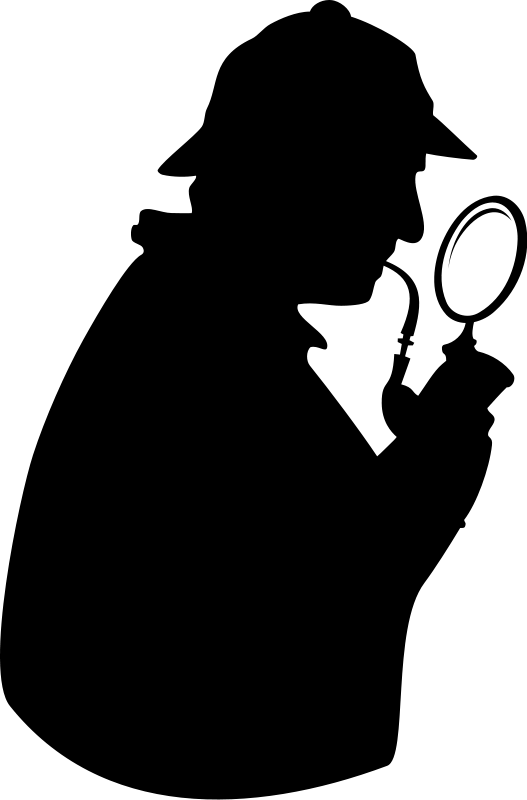
\includegraphics[width=\textwidth]{Metodos/sherlock_holmes}
    \end{column}
    \begin{column}{7.5cm}
      \begin{itemize}
      \item ``Parte de princípios reconhecidos como verdadeiros e
        indiscutíveis e possibilita chegar a conclusões de maneira
        puramente formal, isto é, em virtude unicamente de sua
        lógica.''
      \item Sequência de argumentos lógicos
      \item Ao partir de premissas verdadeiras, chega-se a uma
        conclusão verdadeira
      \item Objetivo: explicar o conteúdo das premissas
      \item Justificativa: ``Só a razão é capaz de levar ao
        conhecimento verdadeiro''
      \end{itemize}
  \end{column}
\end{columns}
\end{frame}

\begin{frame}{Método Dedutivo}
  \begin{example}
    \begin{itemize}
    \item (premissa maior) Todo homem é mortal
    \item (premissa menor) Pedro é homem
    \item (conclusão) Logo, Pedro é mortal
    \end{itemize}
  \end{example}

  \vfill
  Fonte: Prodanov, 2013
\end{frame}

\begin{frame}{Curiosidade: Redução ao absurdo}
  \begin{itemize}
  \item Latim: {\em reductio ad absurdum}
  \item Podemos usar o método dedutivo para ``verificar'' se uma
    premissa é verdadeira:
    \begin{itemize}
    \item \alert{assumindo que ela seja verdadeira}, a conclusão também o será
    \item se a conclusão for falsa (ou ``absurdo'', ou contradição),
      então a premissa não pode ser verdadeira
    \end{itemize}
  \item Ex: ``{\em se todos os seus amigos pularem de uma ponte...}''
  \end{itemize}
\end{frame}

% \begin{frame}{Curiosidade: Redução ao absurdo}
%   \begin{example}
%     \begin{itemize}
%     \item Na Homeopatia, uma premissa central é a de que a água retém
%       memória das substâncias dissolvidas nela


%     \item Na Homeopatia, quanto mais se dinamiza a solução, mais potente ela fica
%     \item Mas dinamizar é diluir 
%     \item Uma solução mais diluída não pode ser mais ``potente''
%       (absurdo!)
%     \end{itemize}
%   \end{example}
% \end{frame}


\subsection{Dedução x Indução}

\begin{frame}{Dedução x Indução}
  \begin{block}{}
    ``The two operations of our understanding, intuition and deduction,
    on which alone we have said we must rely in the acquisition of
    knowledge.''

    René Descartes
  \end{block}
\end{frame}

\begin{frame}{Dedução x Indução}
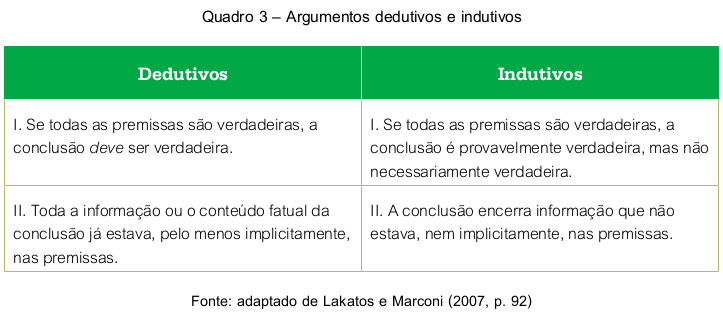
\includegraphics[width=1.05\textwidth]{Metodos/deducao_vs_inducao}
\end{frame}

\begin{frame}{Dedução x Indução}
  \begin{block}{Dedutivo}
    \begin{itemize}
    \item Todo mamífero tem um coração
    \item Todos os cães são mamíferos
    \item Logo, todos os cães tem um coração
    \end{itemize}
  \end{block}
  \begin{block}{Indutivo}
    \begin{itemize}
    \item Todos os cães que foram observados tem um coração
    \item Logo, todos os cães tem um coração
    \end{itemize}
  \end{block}
\end{frame}

\begin{frame}{Dedução x Indução}
  \begin{itemize}
  \item Dedutivo: para que a conclusão fosse falsa, uma das ou as duas
    premissas teriam de ser falsas (ou nem todos os cães são mamíferos
    ou nem todos os mamíferos têm um coração)
  \item Indutivo: é possível que a premissa seja verdadeira e a
    conclusão, falsa (o fato de não ter encontrado um cão sem coração
    não é garantia de que todos os cães tenham um coração)
  \end{itemize}

(Fonte: Prodanov)
\end{frame}

\subsection{Método Hipotético-dedutivo}

\begin{frame}{Método Hipotético-dedutivo}
  \begin{itemize}
  \item Nem sempre podemos generalizar de forma segura (método
    indutivo)
  \item ``o salto indutivo de {\em alguns} para {\em todos} exigiria
    que a observação de fatos isolados atingisse o infinito, o que
    nunca poderia ocorrer, por maior que fosse a quantidade de fatos
    observados'' Karl Popper
  \item Etapas:
    \begin{enumerate}
    \item Problema
    \item Observação
    \item Hipóteses
    \item Tentativa de falseamento
    \item Confirmação ou refutação
    \end{enumerate}
  \end{itemize}
\end{frame}

\begin{frame}{Método Hipotético-dedutivo}
  \begin{center}
    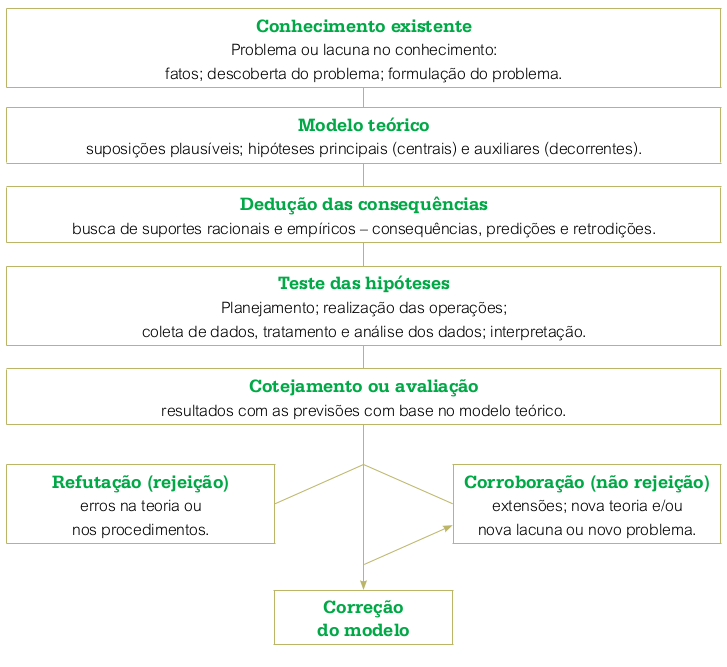
\includegraphics[height=0.95\textheight]{Metodos/metodo_hipotetico}
  \end{center}
\end{frame}

\begin{frame}{Método Hipotético-dedutivo}
  \begin{itemize}
  \item Problema: lacunas na teoria existente.
  \item Solução: nova conjectura deduzida a partir das hipóteses a ser
    testadas
  \item Testes de falseamento: tentativas de refutar as hipóteses pela
    observação e/ou experimentação.
  \end{itemize}
\end{frame}


\subsection{Aprofundamento}

\begin{frame}{Aprofundamento}
  \begin{block}{Leitura}
    Livro texto, seção {\bf 2.4.1}.
  \end{block}
  \begin{block}{Vídeo}
    O Método Científico e os Tipos de Pesquisa \href{https://youtu.be/ey9bTshV308}{https://youtu.be/ey9bTshV308}
  \end{block}

\end{frame}
% \section{Outros métodos}

% \begin{frame}{}
%   \begin{itemize}
%   \item 
%   \end{itemize}
% \end{frame}

% \subsection{Método dialético}

% \begin{frame}{}
%   \begin{itemize}
%   \item 
%   \end{itemize}
% \end{frame}

% \subsection{Método fenomenológico}

% \begin{frame}{}
%   \begin{itemize}
%   \item 
%   \end{itemize}
% \end{frame}

% \subsection{Método histórico}



\end{document}
